
% Default to the notebook output style

    


% Inherit from the specified cell style.




    
\documentclass[11pt]{article}

    
    
    \usepackage[T1]{fontenc}
    % Nicer default font (+ math font) than Computer Modern for most use cases
    \usepackage{mathpazo}

    % Basic figure setup, for now with no caption control since it's done
    % automatically by Pandoc (which extracts ![](path) syntax from Markdown).
    \usepackage{graphicx}
    % We will generate all images so they have a width \maxwidth. This means
    % that they will get their normal width if they fit onto the page, but
    % are scaled down if they would overflow the margins.
    \makeatletter
    \def\maxwidth{\ifdim\Gin@nat@width>\linewidth\linewidth
    \else\Gin@nat@width\fi}
    \makeatother
    \let\Oldincludegraphics\includegraphics
    % Set max figure width to be 80% of text width, for now hardcoded.
    \renewcommand{\includegraphics}[1]{\Oldincludegraphics[width=.8\maxwidth]{#1}}
    % Ensure that by default, figures have no caption (until we provide a
    % proper Figure object with a Caption API and a way to capture that
    % in the conversion process - todo).
    \usepackage{caption}
    \DeclareCaptionLabelFormat{nolabel}{}
    \captionsetup{labelformat=nolabel}

    \usepackage{adjustbox} % Used to constrain images to a maximum size 
    \usepackage{xcolor} % Allow colors to be defined
    \usepackage{enumerate} % Needed for markdown enumerations to work
    \usepackage{geometry} % Used to adjust the document margins
    \usepackage{amsmath} % Equations
    \usepackage{amssymb} % Equations
    \usepackage{textcomp} % defines textquotesingle
    % Hack from http://tex.stackexchange.com/a/47451/13684:
    \AtBeginDocument{%
        \def\PYZsq{\textquotesingle}% Upright quotes in Pygmentized code
    }
    \usepackage{upquote} % Upright quotes for verbatim code
    \usepackage{eurosym} % defines \euro
    \usepackage[mathletters]{ucs} % Extended unicode (utf-8) support
    \usepackage[utf8x]{inputenc} % Allow utf-8 characters in the tex document
    \usepackage{fancyvrb} % verbatim replacement that allows latex
    \usepackage{grffile} % extends the file name processing of package graphics 
                         % to support a larger range 
    % The hyperref package gives us a pdf with properly built
    % internal navigation ('pdf bookmarks' for the table of contents,
    % internal cross-reference links, web links for URLs, etc.)
    \usepackage{hyperref}
    \usepackage{longtable} % longtable support required by pandoc >1.10
    \usepackage{booktabs}  % table support for pandoc > 1.12.2
    \usepackage[inline]{enumitem} % IRkernel/repr support (it uses the enumerate* environment)
    \usepackage[normalem]{ulem} % ulem is needed to support strikethroughs (\sout)
                                % normalem makes italics be italics, not underlines
    

    
    
    % Colors for the hyperref package
    \definecolor{urlcolor}{rgb}{0,.145,.698}
    \definecolor{linkcolor}{rgb}{.71,0.21,0.01}
    \definecolor{citecolor}{rgb}{.12,.54,.11}

    % ANSI colors
    \definecolor{ansi-black}{HTML}{3E424D}
    \definecolor{ansi-black-intense}{HTML}{282C36}
    \definecolor{ansi-red}{HTML}{E75C58}
    \definecolor{ansi-red-intense}{HTML}{B22B31}
    \definecolor{ansi-green}{HTML}{00A250}
    \definecolor{ansi-green-intense}{HTML}{007427}
    \definecolor{ansi-yellow}{HTML}{DDB62B}
    \definecolor{ansi-yellow-intense}{HTML}{B27D12}
    \definecolor{ansi-blue}{HTML}{208FFB}
    \definecolor{ansi-blue-intense}{HTML}{0065CA}
    \definecolor{ansi-magenta}{HTML}{D160C4}
    \definecolor{ansi-magenta-intense}{HTML}{A03196}
    \definecolor{ansi-cyan}{HTML}{60C6C8}
    \definecolor{ansi-cyan-intense}{HTML}{258F8F}
    \definecolor{ansi-white}{HTML}{C5C1B4}
    \definecolor{ansi-white-intense}{HTML}{A1A6B2}

    % commands and environments needed by pandoc snippets
    % extracted from the output of `pandoc -s`
    \providecommand{\tightlist}{%
      \setlength{\itemsep}{0pt}\setlength{\parskip}{0pt}}
    \DefineVerbatimEnvironment{Highlighting}{Verbatim}{commandchars=\\\{\}}
    % Add ',fontsize=\small' for more characters per line
    \newenvironment{Shaded}{}{}
    \newcommand{\KeywordTok}[1]{\textcolor[rgb]{0.00,0.44,0.13}{\textbf{{#1}}}}
    \newcommand{\DataTypeTok}[1]{\textcolor[rgb]{0.56,0.13,0.00}{{#1}}}
    \newcommand{\DecValTok}[1]{\textcolor[rgb]{0.25,0.63,0.44}{{#1}}}
    \newcommand{\BaseNTok}[1]{\textcolor[rgb]{0.25,0.63,0.44}{{#1}}}
    \newcommand{\FloatTok}[1]{\textcolor[rgb]{0.25,0.63,0.44}{{#1}}}
    \newcommand{\CharTok}[1]{\textcolor[rgb]{0.25,0.44,0.63}{{#1}}}
    \newcommand{\StringTok}[1]{\textcolor[rgb]{0.25,0.44,0.63}{{#1}}}
    \newcommand{\CommentTok}[1]{\textcolor[rgb]{0.38,0.63,0.69}{\textit{{#1}}}}
    \newcommand{\OtherTok}[1]{\textcolor[rgb]{0.00,0.44,0.13}{{#1}}}
    \newcommand{\AlertTok}[1]{\textcolor[rgb]{1.00,0.00,0.00}{\textbf{{#1}}}}
    \newcommand{\FunctionTok}[1]{\textcolor[rgb]{0.02,0.16,0.49}{{#1}}}
    \newcommand{\RegionMarkerTok}[1]{{#1}}
    \newcommand{\ErrorTok}[1]{\textcolor[rgb]{1.00,0.00,0.00}{\textbf{{#1}}}}
    \newcommand{\NormalTok}[1]{{#1}}
    
    % Additional commands for more recent versions of Pandoc
    \newcommand{\ConstantTok}[1]{\textcolor[rgb]{0.53,0.00,0.00}{{#1}}}
    \newcommand{\SpecialCharTok}[1]{\textcolor[rgb]{0.25,0.44,0.63}{{#1}}}
    \newcommand{\VerbatimStringTok}[1]{\textcolor[rgb]{0.25,0.44,0.63}{{#1}}}
    \newcommand{\SpecialStringTok}[1]{\textcolor[rgb]{0.73,0.40,0.53}{{#1}}}
    \newcommand{\ImportTok}[1]{{#1}}
    \newcommand{\DocumentationTok}[1]{\textcolor[rgb]{0.73,0.13,0.13}{\textit{{#1}}}}
    \newcommand{\AnnotationTok}[1]{\textcolor[rgb]{0.38,0.63,0.69}{\textbf{\textit{{#1}}}}}
    \newcommand{\CommentVarTok}[1]{\textcolor[rgb]{0.38,0.63,0.69}{\textbf{\textit{{#1}}}}}
    \newcommand{\VariableTok}[1]{\textcolor[rgb]{0.10,0.09,0.49}{{#1}}}
    \newcommand{\ControlFlowTok}[1]{\textcolor[rgb]{0.00,0.44,0.13}{\textbf{{#1}}}}
    \newcommand{\OperatorTok}[1]{\textcolor[rgb]{0.40,0.40,0.40}{{#1}}}
    \newcommand{\BuiltInTok}[1]{{#1}}
    \newcommand{\ExtensionTok}[1]{{#1}}
    \newcommand{\PreprocessorTok}[1]{\textcolor[rgb]{0.74,0.48,0.00}{{#1}}}
    \newcommand{\AttributeTok}[1]{\textcolor[rgb]{0.49,0.56,0.16}{{#1}}}
    \newcommand{\InformationTok}[1]{\textcolor[rgb]{0.38,0.63,0.69}{\textbf{\textit{{#1}}}}}
    \newcommand{\WarningTok}[1]{\textcolor[rgb]{0.38,0.63,0.69}{\textbf{\textit{{#1}}}}}
    
    
    % Define a nice break command that doesn't care if a line doesn't already
    % exist.
    \def\br{\hspace*{\fill} \\* }
    % Math Jax compatability definitions
    \def\gt{>}
    \def\lt{<}
    % Document parameters
    \title{Tutorial-1.2-Probabilistic\_and\_Boolean\_approaches}
    
    
    

    % Pygments definitions
    
\makeatletter
\def\PY@reset{\let\PY@it=\relax \let\PY@bf=\relax%
    \let\PY@ul=\relax \let\PY@tc=\relax%
    \let\PY@bc=\relax \let\PY@ff=\relax}
\def\PY@tok#1{\csname PY@tok@#1\endcsname}
\def\PY@toks#1+{\ifx\relax#1\empty\else%
    \PY@tok{#1}\expandafter\PY@toks\fi}
\def\PY@do#1{\PY@bc{\PY@tc{\PY@ul{%
    \PY@it{\PY@bf{\PY@ff{#1}}}}}}}
\def\PY#1#2{\PY@reset\PY@toks#1+\relax+\PY@do{#2}}

\expandafter\def\csname PY@tok@w\endcsname{\def\PY@tc##1{\textcolor[rgb]{0.73,0.73,0.73}{##1}}}
\expandafter\def\csname PY@tok@c\endcsname{\let\PY@it=\textit\def\PY@tc##1{\textcolor[rgb]{0.25,0.50,0.50}{##1}}}
\expandafter\def\csname PY@tok@cp\endcsname{\def\PY@tc##1{\textcolor[rgb]{0.74,0.48,0.00}{##1}}}
\expandafter\def\csname PY@tok@k\endcsname{\let\PY@bf=\textbf\def\PY@tc##1{\textcolor[rgb]{0.00,0.50,0.00}{##1}}}
\expandafter\def\csname PY@tok@kp\endcsname{\def\PY@tc##1{\textcolor[rgb]{0.00,0.50,0.00}{##1}}}
\expandafter\def\csname PY@tok@kt\endcsname{\def\PY@tc##1{\textcolor[rgb]{0.69,0.00,0.25}{##1}}}
\expandafter\def\csname PY@tok@o\endcsname{\def\PY@tc##1{\textcolor[rgb]{0.40,0.40,0.40}{##1}}}
\expandafter\def\csname PY@tok@ow\endcsname{\let\PY@bf=\textbf\def\PY@tc##1{\textcolor[rgb]{0.67,0.13,1.00}{##1}}}
\expandafter\def\csname PY@tok@nb\endcsname{\def\PY@tc##1{\textcolor[rgb]{0.00,0.50,0.00}{##1}}}
\expandafter\def\csname PY@tok@nf\endcsname{\def\PY@tc##1{\textcolor[rgb]{0.00,0.00,1.00}{##1}}}
\expandafter\def\csname PY@tok@nc\endcsname{\let\PY@bf=\textbf\def\PY@tc##1{\textcolor[rgb]{0.00,0.00,1.00}{##1}}}
\expandafter\def\csname PY@tok@nn\endcsname{\let\PY@bf=\textbf\def\PY@tc##1{\textcolor[rgb]{0.00,0.00,1.00}{##1}}}
\expandafter\def\csname PY@tok@ne\endcsname{\let\PY@bf=\textbf\def\PY@tc##1{\textcolor[rgb]{0.82,0.25,0.23}{##1}}}
\expandafter\def\csname PY@tok@nv\endcsname{\def\PY@tc##1{\textcolor[rgb]{0.10,0.09,0.49}{##1}}}
\expandafter\def\csname PY@tok@no\endcsname{\def\PY@tc##1{\textcolor[rgb]{0.53,0.00,0.00}{##1}}}
\expandafter\def\csname PY@tok@nl\endcsname{\def\PY@tc##1{\textcolor[rgb]{0.63,0.63,0.00}{##1}}}
\expandafter\def\csname PY@tok@ni\endcsname{\let\PY@bf=\textbf\def\PY@tc##1{\textcolor[rgb]{0.60,0.60,0.60}{##1}}}
\expandafter\def\csname PY@tok@na\endcsname{\def\PY@tc##1{\textcolor[rgb]{0.49,0.56,0.16}{##1}}}
\expandafter\def\csname PY@tok@nt\endcsname{\let\PY@bf=\textbf\def\PY@tc##1{\textcolor[rgb]{0.00,0.50,0.00}{##1}}}
\expandafter\def\csname PY@tok@nd\endcsname{\def\PY@tc##1{\textcolor[rgb]{0.67,0.13,1.00}{##1}}}
\expandafter\def\csname PY@tok@s\endcsname{\def\PY@tc##1{\textcolor[rgb]{0.73,0.13,0.13}{##1}}}
\expandafter\def\csname PY@tok@sd\endcsname{\let\PY@it=\textit\def\PY@tc##1{\textcolor[rgb]{0.73,0.13,0.13}{##1}}}
\expandafter\def\csname PY@tok@si\endcsname{\let\PY@bf=\textbf\def\PY@tc##1{\textcolor[rgb]{0.73,0.40,0.53}{##1}}}
\expandafter\def\csname PY@tok@se\endcsname{\let\PY@bf=\textbf\def\PY@tc##1{\textcolor[rgb]{0.73,0.40,0.13}{##1}}}
\expandafter\def\csname PY@tok@sr\endcsname{\def\PY@tc##1{\textcolor[rgb]{0.73,0.40,0.53}{##1}}}
\expandafter\def\csname PY@tok@ss\endcsname{\def\PY@tc##1{\textcolor[rgb]{0.10,0.09,0.49}{##1}}}
\expandafter\def\csname PY@tok@sx\endcsname{\def\PY@tc##1{\textcolor[rgb]{0.00,0.50,0.00}{##1}}}
\expandafter\def\csname PY@tok@m\endcsname{\def\PY@tc##1{\textcolor[rgb]{0.40,0.40,0.40}{##1}}}
\expandafter\def\csname PY@tok@gh\endcsname{\let\PY@bf=\textbf\def\PY@tc##1{\textcolor[rgb]{0.00,0.00,0.50}{##1}}}
\expandafter\def\csname PY@tok@gu\endcsname{\let\PY@bf=\textbf\def\PY@tc##1{\textcolor[rgb]{0.50,0.00,0.50}{##1}}}
\expandafter\def\csname PY@tok@gd\endcsname{\def\PY@tc##1{\textcolor[rgb]{0.63,0.00,0.00}{##1}}}
\expandafter\def\csname PY@tok@gi\endcsname{\def\PY@tc##1{\textcolor[rgb]{0.00,0.63,0.00}{##1}}}
\expandafter\def\csname PY@tok@gr\endcsname{\def\PY@tc##1{\textcolor[rgb]{1.00,0.00,0.00}{##1}}}
\expandafter\def\csname PY@tok@ge\endcsname{\let\PY@it=\textit}
\expandafter\def\csname PY@tok@gs\endcsname{\let\PY@bf=\textbf}
\expandafter\def\csname PY@tok@gp\endcsname{\let\PY@bf=\textbf\def\PY@tc##1{\textcolor[rgb]{0.00,0.00,0.50}{##1}}}
\expandafter\def\csname PY@tok@go\endcsname{\def\PY@tc##1{\textcolor[rgb]{0.53,0.53,0.53}{##1}}}
\expandafter\def\csname PY@tok@gt\endcsname{\def\PY@tc##1{\textcolor[rgb]{0.00,0.27,0.87}{##1}}}
\expandafter\def\csname PY@tok@err\endcsname{\def\PY@bc##1{\setlength{\fboxsep}{0pt}\fcolorbox[rgb]{1.00,0.00,0.00}{1,1,1}{\strut ##1}}}
\expandafter\def\csname PY@tok@kc\endcsname{\let\PY@bf=\textbf\def\PY@tc##1{\textcolor[rgb]{0.00,0.50,0.00}{##1}}}
\expandafter\def\csname PY@tok@kd\endcsname{\let\PY@bf=\textbf\def\PY@tc##1{\textcolor[rgb]{0.00,0.50,0.00}{##1}}}
\expandafter\def\csname PY@tok@kn\endcsname{\let\PY@bf=\textbf\def\PY@tc##1{\textcolor[rgb]{0.00,0.50,0.00}{##1}}}
\expandafter\def\csname PY@tok@kr\endcsname{\let\PY@bf=\textbf\def\PY@tc##1{\textcolor[rgb]{0.00,0.50,0.00}{##1}}}
\expandafter\def\csname PY@tok@bp\endcsname{\def\PY@tc##1{\textcolor[rgb]{0.00,0.50,0.00}{##1}}}
\expandafter\def\csname PY@tok@fm\endcsname{\def\PY@tc##1{\textcolor[rgb]{0.00,0.00,1.00}{##1}}}
\expandafter\def\csname PY@tok@vc\endcsname{\def\PY@tc##1{\textcolor[rgb]{0.10,0.09,0.49}{##1}}}
\expandafter\def\csname PY@tok@vg\endcsname{\def\PY@tc##1{\textcolor[rgb]{0.10,0.09,0.49}{##1}}}
\expandafter\def\csname PY@tok@vi\endcsname{\def\PY@tc##1{\textcolor[rgb]{0.10,0.09,0.49}{##1}}}
\expandafter\def\csname PY@tok@vm\endcsname{\def\PY@tc##1{\textcolor[rgb]{0.10,0.09,0.49}{##1}}}
\expandafter\def\csname PY@tok@sa\endcsname{\def\PY@tc##1{\textcolor[rgb]{0.73,0.13,0.13}{##1}}}
\expandafter\def\csname PY@tok@sb\endcsname{\def\PY@tc##1{\textcolor[rgb]{0.73,0.13,0.13}{##1}}}
\expandafter\def\csname PY@tok@sc\endcsname{\def\PY@tc##1{\textcolor[rgb]{0.73,0.13,0.13}{##1}}}
\expandafter\def\csname PY@tok@dl\endcsname{\def\PY@tc##1{\textcolor[rgb]{0.73,0.13,0.13}{##1}}}
\expandafter\def\csname PY@tok@s2\endcsname{\def\PY@tc##1{\textcolor[rgb]{0.73,0.13,0.13}{##1}}}
\expandafter\def\csname PY@tok@sh\endcsname{\def\PY@tc##1{\textcolor[rgb]{0.73,0.13,0.13}{##1}}}
\expandafter\def\csname PY@tok@s1\endcsname{\def\PY@tc##1{\textcolor[rgb]{0.73,0.13,0.13}{##1}}}
\expandafter\def\csname PY@tok@mb\endcsname{\def\PY@tc##1{\textcolor[rgb]{0.40,0.40,0.40}{##1}}}
\expandafter\def\csname PY@tok@mf\endcsname{\def\PY@tc##1{\textcolor[rgb]{0.40,0.40,0.40}{##1}}}
\expandafter\def\csname PY@tok@mh\endcsname{\def\PY@tc##1{\textcolor[rgb]{0.40,0.40,0.40}{##1}}}
\expandafter\def\csname PY@tok@mi\endcsname{\def\PY@tc##1{\textcolor[rgb]{0.40,0.40,0.40}{##1}}}
\expandafter\def\csname PY@tok@il\endcsname{\def\PY@tc##1{\textcolor[rgb]{0.40,0.40,0.40}{##1}}}
\expandafter\def\csname PY@tok@mo\endcsname{\def\PY@tc##1{\textcolor[rgb]{0.40,0.40,0.40}{##1}}}
\expandafter\def\csname PY@tok@ch\endcsname{\let\PY@it=\textit\def\PY@tc##1{\textcolor[rgb]{0.25,0.50,0.50}{##1}}}
\expandafter\def\csname PY@tok@cm\endcsname{\let\PY@it=\textit\def\PY@tc##1{\textcolor[rgb]{0.25,0.50,0.50}{##1}}}
\expandafter\def\csname PY@tok@cpf\endcsname{\let\PY@it=\textit\def\PY@tc##1{\textcolor[rgb]{0.25,0.50,0.50}{##1}}}
\expandafter\def\csname PY@tok@c1\endcsname{\let\PY@it=\textit\def\PY@tc##1{\textcolor[rgb]{0.25,0.50,0.50}{##1}}}
\expandafter\def\csname PY@tok@cs\endcsname{\let\PY@it=\textit\def\PY@tc##1{\textcolor[rgb]{0.25,0.50,0.50}{##1}}}

\def\PYZbs{\char`\\}
\def\PYZus{\char`\_}
\def\PYZob{\char`\{}
\def\PYZcb{\char`\}}
\def\PYZca{\char`\^}
\def\PYZam{\char`\&}
\def\PYZlt{\char`\<}
\def\PYZgt{\char`\>}
\def\PYZsh{\char`\#}
\def\PYZpc{\char`\%}
\def\PYZdl{\char`\$}
\def\PYZhy{\char`\-}
\def\PYZsq{\char`\'}
\def\PYZdq{\char`\"}
\def\PYZti{\char`\~}
% for compatibility with earlier versions
\def\PYZat{@}
\def\PYZlb{[}
\def\PYZrb{]}
\makeatother


    % Exact colors from NB
    \definecolor{incolor}{rgb}{0.0, 0.0, 0.5}
    \definecolor{outcolor}{rgb}{0.545, 0.0, 0.0}



    
    % Prevent overflowing lines due to hard-to-break entities
    \sloppy 
    % Setup hyperref package
    \hypersetup{
      breaklinks=true,  % so long urls are correctly broken across lines
      colorlinks=true,
      urlcolor=urlcolor,
      linkcolor=linkcolor,
      citecolor=citecolor,
      }
    % Slightly bigger margins than the latex defaults
    
    \geometry{verbose,tmargin=1in,bmargin=1in,lmargin=1in,rmargin=1in}
    
    

    \begin{document}
    
    
    \maketitle
    
    

    
    \section{Define the species interaction
network}\label{define-the-species-interaction-network}

We wish to define the species interaction network used in the example in
the paper. We can define the network by the species present
(\texttt{s1}, \texttt{s2}, etc. below), the interactions between them,
and the signs of these interactions.

    \begin{Verbatim}[commandchars=\\\{\}]
{\color{incolor}In [{\color{incolor}8}]:} \PY{c+c1}{\PYZsh{} spp\PYZus{}list = [\PYZsq{}s1\PYZsq{},\PYZsq{}s2\PYZsq{},\PYZsq{}s3\PYZsq{},\PYZsq{}s4\PYZsq{},\PYZsq{}s5\PYZsq{}]}
        
        \PY{c+c1}{\PYZsh{} key is recipient of a positive effect}
        \PY{n}{positive\PYZus{}edges\PYZus{}dict} \PY{o}{=} \PY{p}{\PYZob{}}
        \PY{l+s+s1}{\PYZsq{}}\PY{l+s+s1}{s5}\PY{l+s+s1}{\PYZsq{}}\PY{p}{:} \PY{p}{[}\PY{l+s+s1}{\PYZsq{}}\PY{l+s+s1}{s4}\PY{l+s+s1}{\PYZsq{}}\PY{p}{]}\PY{p}{,}
        \PY{l+s+s1}{\PYZsq{}}\PY{l+s+s1}{s3}\PY{l+s+s1}{\PYZsq{}}\PY{p}{:} \PY{p}{[}\PY{l+s+s1}{\PYZsq{}}\PY{l+s+s1}{s2}\PY{l+s+s1}{\PYZsq{}}\PY{p}{,} \PY{l+s+s1}{\PYZsq{}}\PY{l+s+s1}{s4}\PY{l+s+s1}{\PYZsq{}}\PY{p}{,} \PY{l+s+s1}{\PYZsq{}}\PY{l+s+s1}{s5}\PY{l+s+s1}{\PYZsq{}}\PY{p}{]}\PY{p}{,}
        \PY{p}{\PYZcb{}}
        
        \PY{c+c1}{\PYZsh{} key is recipient of a negative effect}
        \PY{n}{negative\PYZus{}edges\PYZus{}dict} \PY{o}{=} \PY{p}{\PYZob{}}
        \PY{l+s+s1}{\PYZsq{}}\PY{l+s+s1}{s5}\PY{l+s+s1}{\PYZsq{}}\PY{p}{:} \PY{p}{[}\PY{l+s+s1}{\PYZsq{}}\PY{l+s+s1}{s5}\PY{l+s+s1}{\PYZsq{}}\PY{p}{]}\PY{p}{,}
        \PY{l+s+s1}{\PYZsq{}}\PY{l+s+s1}{s4}\PY{l+s+s1}{\PYZsq{}}\PY{p}{:} \PY{p}{[}\PY{l+s+s1}{\PYZsq{}}\PY{l+s+s1}{s4}\PY{l+s+s1}{\PYZsq{}}\PY{p}{,} \PY{l+s+s1}{\PYZsq{}}\PY{l+s+s1}{s5}\PY{l+s+s1}{\PYZsq{}}\PY{p}{,} \PY{l+s+s1}{\PYZsq{}}\PY{l+s+s1}{s3}\PY{l+s+s1}{\PYZsq{}}\PY{p}{]}\PY{p}{,}
        \PY{l+s+s1}{\PYZsq{}}\PY{l+s+s1}{s3}\PY{l+s+s1}{\PYZsq{}}\PY{p}{:} \PY{p}{[}\PY{l+s+s1}{\PYZsq{}}\PY{l+s+s1}{s3}\PY{l+s+s1}{\PYZsq{}}\PY{p}{]}\PY{p}{,}
        \PY{l+s+s1}{\PYZsq{}}\PY{l+s+s1}{s2}\PY{l+s+s1}{\PYZsq{}}\PY{p}{:} \PY{p}{[}\PY{l+s+s1}{\PYZsq{}}\PY{l+s+s1}{s2}\PY{l+s+s1}{\PYZsq{}}\PY{p}{,} \PY{l+s+s1}{\PYZsq{}}\PY{l+s+s1}{s1}\PY{l+s+s1}{\PYZsq{}}\PY{p}{,} \PY{l+s+s1}{\PYZsq{}}\PY{l+s+s1}{s3}\PY{l+s+s1}{\PYZsq{}}\PY{p}{]}\PY{p}{,}
        \PY{l+s+s1}{\PYZsq{}}\PY{l+s+s1}{s1}\PY{l+s+s1}{\PYZsq{}}\PY{p}{:} \PY{p}{[}\PY{l+s+s1}{\PYZsq{}}\PY{l+s+s1}{s1}\PY{l+s+s1}{\PYZsq{}}\PY{p}{,} \PY{l+s+s1}{\PYZsq{}}\PY{l+s+s1}{s2}\PY{l+s+s1}{\PYZsq{}}\PY{p}{]}\PY{p}{,}
        \PY{p}{\PYZcb{}}
\end{Verbatim}


    The network structure is encoded as a \texttt{networkx} digraph. The
function \texttt{initialise\_foodweb} stores the signs of the
interactions in the edge data dictionary.

    \begin{Verbatim}[commandchars=\\\{\}]
{\color{incolor}In [{\color{incolor}9}]:} \PY{k+kn}{from} \PY{n+nn}{qualmod} \PY{k}{import} \PY{n}{initialise\PYZus{}foodweb}
        
        \PY{n}{web} \PY{o}{=} \PY{n}{initialise\PYZus{}foodweb}\PY{p}{(}\PY{n}{positive\PYZus{}edges\PYZus{}dict}\PY{p}{,} \PY{n}{negative\PYZus{}edges\PYZus{}dict}\PY{p}{)}
        
        \PY{c+c1}{\PYZsh{} print edges}
        \PY{k}{for} \PY{n}{edge} \PY{o+ow}{in} \PY{n}{web}\PY{o}{.}\PY{n}{edges}\PY{p}{(}\PY{n}{data}\PY{o}{=}\PY{k+kc}{True}\PY{p}{)}\PY{p}{:}
            \PY{n+nb}{print}\PY{p}{(}\PY{n}{edge}\PY{p}{)}
\end{Verbatim}


    \begin{Verbatim}[commandchars=\\\{\}]
('s5', 's5', \{'color': 'red', 'sign': -1\})
('s5', 's4', \{'color': 'red', 'sign': -1\})
('s5', 's3', \{'color': 'green', 'sign': 1\})
('s4', 's4', \{'color': 'red', 'sign': -1\})
('s4', 's5', \{'color': 'green', 'sign': 1\})
('s4', 's3', \{'color': 'green', 'sign': 1\})
('s3', 's4', \{'color': 'red', 'sign': -1\})
('s3', 's3', \{'color': 'red', 'sign': -1\})
('s3', 's2', \{'color': 'red', 'sign': -1\})
('s2', 's2', \{'color': 'red', 'sign': -1\})
('s2', 's1', \{'color': 'red', 'sign': -1\})
('s2', 's3', \{'color': 'green', 'sign': 1\})
('s1', 's2', \{'color': 'red', 'sign': -1\})
('s1', 's1', \{'color': 'red', 'sign': -1\})

    \end{Verbatim}

    The package \texttt{networkx} provides a quick way to plot the
interaction network.

    \begin{Verbatim}[commandchars=\\\{\}]
{\color{incolor}In [{\color{incolor}10}]:} \PY{k+kn}{import} \PY{n+nn}{networkx} \PY{k}{as} \PY{n+nn}{nx}
         \PY{k+kn}{import} \PY{n+nn}{matplotlib}\PY{n+nn}{.}\PY{n+nn}{pyplot} \PY{k}{as} \PY{n+nn}{plt}
         
         \PY{n}{pos}\PY{o}{=}\PY{n}{nx}\PY{o}{.}\PY{n}{spring\PYZus{}layout}\PY{p}{(}\PY{n}{web}\PY{p}{)}
         \PY{n}{nx}\PY{o}{.}\PY{n}{draw\PYZus{}networkx\PYZus{}labels}\PY{p}{(}\PY{n}{web}\PY{p}{,} \PY{n}{pos}\PY{p}{)}
         \PY{n}{nx}\PY{o}{.}\PY{n}{draw\PYZus{}networkx\PYZus{}nodes}\PY{p}{(}\PY{n}{web}\PY{p}{,} 
                                \PY{n}{pos}\PY{p}{,} 
                                \PY{n}{node\PYZus{}color} \PY{o}{=} \PY{l+s+s1}{\PYZsq{}}\PY{l+s+s1}{white}\PY{l+s+s1}{\PYZsq{}}\PY{p}{,} 
                                \PY{n}{edgecolors}\PY{o}{=}\PY{l+s+s1}{\PYZsq{}}\PY{l+s+s1}{black}\PY{l+s+s1}{\PYZsq{}}\PY{p}{,} 
                                \PY{n}{node\PYZus{}size}\PY{o}{=}\PY{l+m+mi}{500}\PY{p}{)}
         
         \PY{n}{edge\PYZus{}colors} \PY{o}{=} \PY{p}{[} \PY{n}{v}\PY{p}{[}\PY{l+m+mi}{2}\PY{p}{]}\PY{p}{[}\PY{l+s+s1}{\PYZsq{}}\PY{l+s+s1}{color}\PY{l+s+s1}{\PYZsq{}}\PY{p}{]} \PY{k}{for} \PY{n}{v} \PY{o+ow}{in} \PY{n}{web}\PY{o}{.}\PY{n}{edges}\PY{p}{(}\PY{n}{data}\PY{o}{=}\PY{k+kc}{True}\PY{p}{)} \PY{p}{]}
         \PY{n}{nx}\PY{o}{.}\PY{n}{draw\PYZus{}networkx\PYZus{}edges}\PY{p}{(}\PY{n}{web}\PY{p}{,} 
                                \PY{n}{pos}\PY{p}{,} 
                                \PY{n}{edge\PYZus{}color}\PY{o}{=}\PY{n}{edge\PYZus{}colors}\PY{p}{,} 
                                \PY{n}{arrows}\PY{o}{=}\PY{k+kc}{True}\PY{p}{,} 
                                \PY{n}{arrowsize}\PY{o}{=}\PY{l+m+mi}{40}\PY{p}{)}\PY{p}{;}
         \PY{n}{plt}\PY{o}{.}\PY{n}{show}\PY{p}{(}\PY{p}{)}
\end{Verbatim}


    \begin{center}
    \adjustimage{max size={0.9\linewidth}{0.9\paperheight}}{output_5_0.png}
    \end{center}
    { \hspace*{\fill} \\}
    
    The package \texttt{qualmod} also includes a function that uses
\texttt{graphviz} to draw the interaction network. This is useful if we
want to create a \texttt{.pdf} of the network to embed in a document,
etc.

    \begin{Verbatim}[commandchars=\\\{\}]
{\color{incolor}In [{\color{incolor}11}]:} \PY{k+kn}{from} \PY{n+nn}{qualmod} \PY{k}{import} \PY{n}{draw\PYZus{}foodweb}
         \PY{k+kn}{from} \PY{n+nn}{IPython}\PY{n+nn}{.}\PY{n+nn}{display} \PY{k}{import} \PY{n}{IFrame}
         \PY{k+kn}{from} \PY{n+nn}{IPython}\PY{n+nn}{.}\PY{n+nn}{display} \PY{k}{import} \PY{n}{Image}
         \PY{k+kn}{import} \PY{n+nn}{os}
         
         \PY{c+c1}{\PYZsh{} use draw\PYZus{}foodweb to create a graphviz dot file }
         \PY{c+c1}{\PYZsh{} defining the interaction network}
         \PY{n}{draw\PYZus{}foodweb}\PY{p}{(}\PY{n}{web}\PY{p}{,} \PY{n}{f\PYZus{}name} \PY{o}{=} \PY{l+s+s1}{\PYZsq{}}\PY{l+s+s1}{web.dot}\PY{l+s+s1}{\PYZsq{}}\PY{p}{)}
         
         \PY{c+c1}{\PYZsh{} call graphviz externally to create a pdf of the }
         \PY{c+c1}{\PYZsh{} interaction network}
         \PY{n}{os}\PY{o}{.}\PY{n}{system}\PY{p}{(}\PY{l+s+s2}{\PYZdq{}}\PY{l+s+s2}{dot \PYZhy{}Tpdf web.dot \PYZgt{} web.pdf}\PY{l+s+s2}{\PYZdq{}}\PY{p}{)}
         
         \PY{c+c1}{\PYZsh{} display the pdf of the interaction network here in Jupyter}
         \PY{c+c1}{\PYZsh{} IFrame(\PYZdq{}web.pdf\PYZdq{}, width=500, height=600)}
         
         \PY{c+c1}{\PYZsh{} call graphviz to create a png, display in }
         \PY{c+c1}{\PYZsh{} markdown cell}
         \PY{n}{os}\PY{o}{.}\PY{n}{system}\PY{p}{(}\PY{l+s+s2}{\PYZdq{}}\PY{l+s+s2}{dot \PYZhy{}Tpng web.dot \PYZgt{} web.png}\PY{l+s+s2}{\PYZdq{}}\PY{p}{)}
\end{Verbatim}


\begin{Verbatim}[commandchars=\\\{\}]
{\color{outcolor}Out[{\color{outcolor}11}]:} 0
\end{Verbatim}
            
    \begin{figure}
\centering
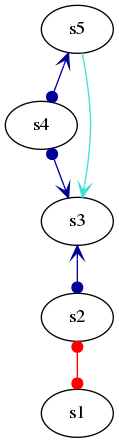
\includegraphics{web.png}
\caption{title}
\end{figure}

\texttt{web.png}

    The interaction network can also be converted into a qualitative
community matrix, \texttt{Mq} below, using the function
\texttt{qualitative\_community\_matrix}.

    \begin{Verbatim}[commandchars=\\\{\}]
{\color{incolor}In [{\color{incolor}12}]:} \PY{k+kn}{from} \PY{n+nn}{qualmod} \PY{k}{import} \PY{n}{qualitative\PYZus{}community\PYZus{}matrix}
         
         \PY{p}{(}\PY{n}{Mq}\PY{p}{,} \PY{n}{s2idx}\PY{p}{)} \PY{o}{=} \PY{n}{qualitative\PYZus{}community\PYZus{}matrix}\PY{p}{(}\PY{n}{web}\PY{p}{)}
         \PY{n+nb}{print}\PY{p}{(}\PY{n}{Mq}\PY{p}{)}
\end{Verbatim}


    \begin{Verbatim}[commandchars=\\\{\}]
[[-1. -1.  0.  0.  0.]
 [-1. -1. -1.  0.  0.]
 [ 0.  1. -1.  1.  1.]
 [ 0.  0. -1. -1. -1.]
 [ 0.  0.  0.  1. -1.]]

    \end{Verbatim}

    The function \texttt{qualitative\_community\_matrix} also returns
\texttt{s2idx}, which is a handy bidirection dictionary that maps the
name of the species to their index in the qualitative community matrix.

    \begin{Verbatim}[commandchars=\\\{\}]
{\color{incolor}In [{\color{incolor}13}]:} \PY{n+nb}{print}\PY{p}{(}\PY{n}{s2idx}\PY{p}{)}
         \PY{n+nb}{print}\PY{p}{(}\PY{n}{s2idx}\PY{p}{[}\PY{l+s+s1}{\PYZsq{}}\PY{l+s+s1}{s1}\PY{l+s+s1}{\PYZsq{}}\PY{p}{]}\PY{p}{)}
         \PY{n+nb}{print}\PY{p}{(}\PY{n}{s2idx}\PY{o}{.}\PY{n}{inv}\PY{p}{[}\PY{l+m+mi}{0}\PY{p}{]}\PY{p}{)}
\end{Verbatim}


    \begin{Verbatim}[commandchars=\\\{\}]
bidict(\{'s1': 0, 's2': 1, 's3': 2, 's4': 3, 's5': 4\})
0
s1

    \end{Verbatim}

    \section{Randomly sampling perturbation responses / parameter
sweep}\label{randomly-sampling-perturbation-responses-parameter-sweep}

In the example in the paper, we are interested in the response of
species \texttt{s3}, \texttt{s4}, and \texttt{s5} to a negative
press-perturbation of species \texttt{s3}.

    \begin{Verbatim}[commandchars=\\\{\}]
{\color{incolor}In [{\color{incolor}14}]:} \PY{c+c1}{\PYZsh{} which species is controlled }
         \PY{c+c1}{\PYZsh{} (i.e. perturbed e.g. by pest control program)}
         \PY{n}{control\PYZus{}list} \PY{o}{=} \PY{p}{[}\PY{l+s+s1}{\PYZsq{}}\PY{l+s+s1}{s3}\PY{l+s+s1}{\PYZsq{}}\PY{p}{]}
         
         \PY{c+c1}{\PYZsh{} the species we\PYZsq{}re interested in the responses of}
         \PY{n}{monitored\PYZus{}list} \PY{o}{=} \PY{p}{[}\PY{l+s+s1}{\PYZsq{}}\PY{l+s+s1}{s3}\PY{l+s+s1}{\PYZsq{}}\PY{p}{,}\PY{l+s+s1}{\PYZsq{}}\PY{l+s+s1}{s4}\PY{l+s+s1}{\PYZsq{}}\PY{p}{,}\PY{l+s+s1}{\PYZsq{}}\PY{l+s+s1}{s5}\PY{l+s+s1}{\PYZsq{}}\PY{p}{]}
\end{Verbatim}


    In probabilistic Qualitative Modelling, the monitored species' response
to the press-perturbation can be obtained using Monte Carlo simulation.
The interaction-strength magnitudes in the community matrix are sampled
from \(a_{i,j} \sim \mathcal{U}(0,1)\), and the positive and negative
responses are counted: \texttt{countResponses} below.

In the Boolean approach, random sampling can also be used to do a
parameter-value sweep of the model behaviour. The objective is to obtain
a set, \texttt{observedResponseCombinations}, that lists every
species-response combination that is possible, regardless of what the
interaction-strength magnitudes are. Here note that, although we again
sample from a uniform distribution, the choice is of distribution is
somewhat arbitrary. So long as we obtain good-enough coverage of the
parameter space that we obtain every possible response combination, then
any sampling distribution can be used.

In this example we apply only one plausibility criterion: the community
matrix must be stable.

The method uses the sensitivity matrix approach to obtain species
responses (\texttt{Sq}).

    \begin{Verbatim}[commandchars=\\\{\}]
{\color{incolor}In [{\color{incolor}15}]:} \PY{k+kn}{import} \PY{n+nn}{numpy} \PY{k}{as} \PY{n+nn}{np}
         
         \PY{n}{sz} \PY{o}{=} \PY{n}{Mq}\PY{o}{.}\PY{n}{shape}\PY{p}{[}\PY{l+m+mi}{0}\PY{p}{]} \PY{c+c1}{\PYZsh{} size of the system, can also use sz = web.order()}
         
         \PY{c+c1}{\PYZsh{} initialise collected responses with empty sets}
         \PY{n}{observedResponseCombinations} \PY{o}{=} \PY{n+nb}{set}\PY{p}{(}\PY{p}{)}
         
         \PY{c+c1}{\PYZsh{} initialise counts of positive responses with zeros}
         \PY{n}{countResponses} \PY{o}{=} \PY{n}{np}\PY{o}{.}\PY{n}{array}\PY{p}{(}\PY{p}{[}\PY{l+m+mi}{0}\PY{p}{]}\PY{o}{*}\PY{n+nb}{len}\PY{p}{(}\PY{n}{control\PYZus{}list}\PY{p}{)}\PY{o}{*}\PY{n+nb}{len}\PY{p}{(}\PY{n}{monitored\PYZus{}list}\PY{p}{)}\PY{p}{)}
         
         \PY{n}{noSamples} \PY{o}{=} \PY{l+m+mi}{100}
         \PY{k}{for} \PY{n}{n} \PY{o+ow}{in} \PY{n+nb}{range}\PY{p}{(}\PY{n}{noSamples}\PY{p}{)}\PY{p}{:} 
             
             \PY{c+c1}{\PYZsh{} find a random community matrix that is stable}
             \PY{n}{maxEig} \PY{o}{=} \PY{l+m+mi}{1}
             \PY{k}{while} \PY{n}{maxEig} \PY{o}{\PYZgt{}} \PY{l+m+mi}{0}\PY{p}{:}
                 
                 \PY{n}{M} \PY{o}{=} \PY{n}{np}\PY{o}{.}\PY{n}{multiply}\PY{p}{(} \PY{n}{np}\PY{o}{.}\PY{n}{random}\PY{o}{.}\PY{n}{random\PYZus{}sample}\PY{p}{(}\PY{p}{(}\PY{n}{sz}\PY{p}{,}\PY{n}{sz}\PY{p}{)}\PY{p}{)}\PY{p}{,} \PY{n}{Mq} \PY{p}{)}
                 \PY{n}{maxEig} \PY{o}{=} \PY{n+nb}{max}\PY{p}{(}\PY{n}{np}\PY{o}{.}\PY{n}{real}\PY{p}{(}\PY{n}{np}\PY{o}{.}\PY{n}{linalg}\PY{o}{.}\PY{n}{eigvals}\PY{p}{(}\PY{n}{M}\PY{p}{)}\PY{p}{)}\PY{p}{)}
                 
             \PY{c+c1}{\PYZsh{} find sensitivity matrix}
             \PY{n}{Sq} \PY{o}{=} \PY{o}{\PYZhy{}} \PY{n}{np}\PY{o}{.}\PY{n}{linalg}\PY{o}{.}\PY{n}{inv}\PY{p}{(}\PY{n}{M}\PY{p}{)}
         
             \PY{c+c1}{\PYZsh{} find the signs of responses of each monitored species }
             \PY{c+c1}{\PYZsh{} to perturbations in each control species}
             \PY{n}{response} \PY{o}{=} \PY{n+nb}{tuple}\PY{p}{(}\PY{p}{[}\PY{l+s+s1}{\PYZsq{}}\PY{l+s+s1}{neg}\PY{l+s+s1}{\PYZsq{}} \PY{k}{if} \PY{n}{Sq}\PY{p}{[}\PY{n}{s2idx}\PY{p}{[}\PY{n}{ms}\PY{p}{]}\PY{p}{,}\PY{n}{s2idx}\PY{p}{[}\PY{n}{cs}\PY{p}{]}\PY{p}{]}\PY{o}{\PYZlt{}}\PY{l+m+mi}{0} \PY{k}{else} \PY{l+s+s1}{\PYZsq{}}\PY{l+s+s1}{pos}\PY{l+s+s1}{\PYZsq{}} 
                               \PY{k}{for} \PY{n}{cs} \PY{o+ow}{in} \PY{n}{control\PYZus{}list} 
                               \PY{k}{for} \PY{n}{ms} \PY{o+ow}{in} \PY{n}{monitored\PYZus{}list} \PY{p}{]}\PY{p}{)}
             \PY{n}{observedResponseCombinations}\PY{o}{.}\PY{n}{add}\PY{p}{(}\PY{n}{response}\PY{p}{)} \PY{c+c1}{\PYZsh{} add to our collection}
             
             \PY{c+c1}{\PYZsh{} add positive responses to count}
             \PY{n}{posResponses} \PY{o}{=} \PY{n}{np}\PY{o}{.}\PY{n}{array}\PY{p}{(}\PY{p}{[} \PY{l+m+mi}{0} \PY{k}{if} \PY{n}{Sq}\PY{p}{[}\PY{n}{s2idx}\PY{p}{[}\PY{n}{ms}\PY{p}{]}\PY{p}{,}\PY{n}{s2idx}\PY{p}{[}\PY{n}{cs}\PY{p}{]}\PY{p}{]}\PY{o}{\PYZlt{}}\PY{l+m+mi}{0} \PY{k}{else} \PY{l+m+mi}{1} 
                                      \PY{k}{for} \PY{n}{cs} \PY{o+ow}{in} \PY{n}{control\PYZus{}list} 
                                      \PY{k}{for} \PY{n}{ms} \PY{o+ow}{in} \PY{n}{monitored\PYZus{}list} \PY{p}{]}\PY{p}{)}
             \PY{n}{countResponses} \PY{o}{+}\PY{o}{=} \PY{n}{posResponses} \PY{c+c1}{\PYZsh{} add to our count}
\end{Verbatim}


    The two types of intermediate results are shown below:

    \begin{Verbatim}[commandchars=\\\{\}]
{\color{incolor}In [{\color{incolor}16}]:} \PY{n}{countResponses}
\end{Verbatim}


\begin{Verbatim}[commandchars=\\\{\}]
{\color{outcolor}Out[{\color{outcolor}16}]:} array([85, 15, 15])
\end{Verbatim}
            
    \begin{Verbatim}[commandchars=\\\{\}]
{\color{incolor}In [{\color{incolor}17}]:} \PY{n}{observedResponseCombinations}
\end{Verbatim}


\begin{Verbatim}[commandchars=\\\{\}]
{\color{outcolor}Out[{\color{outcolor}17}]:} \{('neg', 'pos', 'pos'), ('pos', 'neg', 'neg')\}
\end{Verbatim}
            
    \section{Probabilistic approach}\label{probabilistic-approach}

In the probabilistic approach, the proportions of responses giving
positive or negative species response are interpreted probabilistically.

In this example, probabilistic QM suggests stronger support for a
positive response in species \texttt{s3}, and a negative response in
species \texttt{s4} and \texttt{s5}.

    \begin{Verbatim}[commandchars=\\\{\}]
{\color{incolor}In [{\color{incolor}18}]:} \PY{n}{probabilityResponses} \PY{o}{=} \PY{n}{countResponses} \PY{o}{/} \PY{n}{noSamples}
         
         \PY{n}{plt}\PY{o}{.}\PY{n}{title}\PY{p}{(}\PY{l+s+s1}{\PYZsq{}}\PY{l+s+s1}{responses to a negative press perturbation of s3}\PY{l+s+s1}{\PYZsq{}}\PY{p}{)}
         \PY{n}{plt}\PY{o}{.}\PY{n}{bar}\PY{p}{(}\PY{n+nb}{range}\PY{p}{(}\PY{n+nb}{len}\PY{p}{(}\PY{n}{monitored\PYZus{}list}\PY{p}{)}\PY{p}{)}\PY{p}{,} 
                 \PY{n}{probabilityResponses}\PY{p}{,} 
                 \PY{n}{tick\PYZus{}label}\PY{o}{=}\PY{n}{monitored\PYZus{}list}\PY{p}{)}
         \PY{n}{plt}\PY{o}{.}\PY{n}{ylim}\PY{p}{(}\PY{p}{(}\PY{l+m+mi}{0}\PY{p}{,}\PY{l+m+mi}{1}\PY{p}{)}\PY{p}{)}
         \PY{n}{plt}\PY{o}{.}\PY{n}{ylabel}\PY{p}{(}\PY{l+s+s1}{\PYZsq{}}\PY{l+s+s1}{probability of a positive response}\PY{l+s+s1}{\PYZsq{}}\PY{p}{)}
         \PY{n}{plt}\PY{o}{.}\PY{n}{xlabel}\PY{p}{(}\PY{l+s+s1}{\PYZsq{}}\PY{l+s+s1}{species}\PY{l+s+s1}{\PYZsq{}}\PY{p}{)}
         \PY{n}{plt}\PY{o}{.}\PY{n}{show}\PY{p}{(}\PY{p}{)}
\end{Verbatim}


    \begin{center}
    \adjustimage{max size={0.9\linewidth}{0.9\paperheight}}{output_21_0.png}
    \end{center}
    { \hspace*{\fill} \\}
    
    \section{Boolean approach}\label{boolean-approach}

In the Boolean approach, the species response-combinations that the
model predicts are interpreted using Boolean algebra.

Two species-response combinations were observed during the
parameter-value sweep (shown as a table below). It assumed that
parameter sweep above was sufficient to obtain every possible
combination.

    \begin{Verbatim}[commandchars=\\\{\}]
{\color{incolor}In [{\color{incolor}19}]:} \PY{c+c1}{\PYZsh{} the responses we\PYZsq{}ll be counting proportions on}
         \PY{n}{desiredResponses} \PY{o}{=} \PY{p}{[} \PY{n}{cs} \PY{o}{+} \PY{l+s+s1}{\PYZsq{}}\PY{l+s+s1}{\PYZus{}}\PY{l+s+s1}{\PYZsq{}} \PY{o}{+} \PY{n}{ms} 
                             \PY{k}{for} \PY{n}{cs} \PY{o+ow}{in} \PY{n}{control\PYZus{}list} 
                             \PY{k}{for} \PY{n}{ms} \PY{o+ow}{in} \PY{n}{monitored\PYZus{}list}\PY{p}{]}
         
         \PY{c+c1}{\PYZsh{} I have hardcoded the answer in here in case, by chance, }
         \PY{c+c1}{\PYZsh{} you miss a response combination in the random sampling above.}
         \PY{c+c1}{\PYZsh{} For a real example, you will need to check that a large no. }
         \PY{c+c1}{\PYZsh{} of samples has been drawn since the last new response }
         \PY{c+c1}{\PYZsh{} combination was found.}
         
         \PY{k}{if} \PY{n+nb}{len}\PY{p}{(}\PY{n}{observedResponseCombinations}\PY{p}{)} \PY{o}{\PYZlt{}} \PY{l+m+mi}{2}\PY{p}{:}
             \PY{n}{observedResponseCombinations} \PY{o}{=} \PY{p}{\PYZob{}}
                 \PY{p}{(}\PY{l+s+s1}{\PYZsq{}}\PY{l+s+s1}{neg}\PY{l+s+s1}{\PYZsq{}}\PY{p}{,} \PY{l+s+s1}{\PYZsq{}}\PY{l+s+s1}{pos}\PY{l+s+s1}{\PYZsq{}}\PY{p}{,} \PY{l+s+s1}{\PYZsq{}}\PY{l+s+s1}{pos}\PY{l+s+s1}{\PYZsq{}}\PY{p}{)}\PY{p}{,} 
                 \PY{p}{(}\PY{l+s+s1}{\PYZsq{}}\PY{l+s+s1}{pos}\PY{l+s+s1}{\PYZsq{}}\PY{p}{,} \PY{l+s+s1}{\PYZsq{}}\PY{l+s+s1}{neg}\PY{l+s+s1}{\PYZsq{}}\PY{p}{,} \PY{l+s+s1}{\PYZsq{}}\PY{l+s+s1}{neg}\PY{l+s+s1}{\PYZsq{}}\PY{p}{)}
             \PY{p}{\PYZcb{}}
         
         \PY{c+c1}{\PYZsh{} print the species response combinations that were observed }
         \PY{c+c1}{\PYZsh{} during the parameter sweep above in a table}
         \PY{n}{header} \PY{o}{=} \PY{l+s+s1}{\PYZsq{}}\PY{l+s+s1}{ | }\PY{l+s+s1}{\PYZsq{}}\PY{o}{.}\PY{n}{join}\PY{p}{(}\PY{n}{desiredResponses}\PY{p}{)}
         \PY{n+nb}{print}\PY{p}{(}\PY{n}{header}\PY{p}{)}
         \PY{n+nb}{print}\PY{p}{(}\PY{l+s+s1}{\PYZsq{}}\PY{l+s+s1}{\PYZhy{}}\PY{l+s+s1}{\PYZsq{}}\PY{o}{*}\PY{n+nb}{len}\PY{p}{(}\PY{n}{header}\PY{p}{)}\PY{p}{)}
         \PY{k}{for} \PY{n}{responseCombination} \PY{o+ow}{in} \PY{n}{observedResponseCombinations}\PY{p}{:}
             \PY{n+nb}{print}\PY{p}{(}\PY{l+s+s1}{\PYZsq{}}\PY{l+s+s1}{ }\PY{l+s+s1}{\PYZsq{}} \PY{o}{+} \PY{l+s+s1}{\PYZsq{}}\PY{l+s+s1}{  |  }\PY{l+s+s1}{\PYZsq{}}\PY{o}{.}\PY{n}{join}\PY{p}{(}\PY{n}{responseCombination}\PY{p}{)}\PY{p}{)}
\end{Verbatim}


    \begin{Verbatim}[commandchars=\\\{\}]
s3\_s3 | s3\_s4 | s3\_s5
---------------------
 pos  |  neg  |  neg
 neg  |  pos  |  pos

    \end{Verbatim}

    In order to use Boolean algebra, we need to convert the species
responses into Boolean values. This is easiest when the responses have a
natural dichotimisation i.e. a positive or a negative species response.
Arbitrarily, we assign a positive species response as a \texttt{true},
and a negative species response as a \texttt{false}.

    \begin{Verbatim}[commandchars=\\\{\}]
{\color{incolor}In [{\color{incolor}20}]:} \PY{n}{str4true} \PY{o}{=} \PY{l+s+s1}{\PYZsq{}}\PY{l+s+s1}{pos}\PY{l+s+s1}{\PYZsq{}}\PY{p}{;} \PY{n}{str4false} \PY{o}{=} \PY{l+s+s1}{\PYZsq{}}\PY{l+s+s1}{neg}\PY{l+s+s1}{\PYZsq{}}
\end{Verbatim}


    The simulations have returned the species-response combinations that are
\emph{possible} in the model, but the Boolean analysis is performed on
the \emph{impossible} combinations instead. Therefore we need to find
the complement of the set of observed responses, i.e. the set of every
response-combination that is combinatorially possible, minus the set of
responses that we observed.

There are a few different ways that we could obtain the complement, but
one convenient way is to first observe that every response combination
can be interpreted as a binary string. Then the complement corresponds
to the list of integers that are missing from the set of integers that
we observed.

Each possible response is encoded as a binary string, and converted into
an integer.

    \begin{Verbatim}[commandchars=\\\{\}]
{\color{incolor}In [{\color{incolor}21}]:} \PY{n}{observedInts} \PY{o}{=} \PY{p}{[} \PY{n+nb}{int}\PY{p}{(}\PY{l+s+s1}{\PYZsq{}}\PY{l+s+s1}{\PYZsq{}}\PY{o}{.}\PY{n}{join}\PY{p}{(}\PY{p}{[}\PY{l+s+s1}{\PYZsq{}}\PY{l+s+s1}{1}\PY{l+s+s1}{\PYZsq{}} \PY{k}{if} \PY{n}{i} \PY{o+ow}{in} \PY{n}{str4true} 
                                       \PY{k}{else} \PY{l+s+s1}{\PYZsq{}}\PY{l+s+s1}{0}\PY{l+s+s1}{\PYZsq{}} \PY{k}{for} \PY{n}{i} \PY{o+ow}{in} \PY{n}{responseCombination}\PY{p}{]}\PY{p}{)}\PY{p}{,} \PY{l+m+mi}{2}\PY{p}{)} 
                         \PY{k}{for} \PY{n}{responseCombination} \PY{o+ow}{in} \PY{n}{observedResponseCombinations} \PY{p}{]}
         \PY{n}{observedInts}
\end{Verbatim}


\begin{Verbatim}[commandchars=\\\{\}]
{\color{outcolor}Out[{\color{outcolor}21}]:} [4, 3]
\end{Verbatim}
            
    Then the unobserved species responses correspond to the integers that
are missing.

    \begin{Verbatim}[commandchars=\\\{\}]
{\color{incolor}In [{\color{incolor}26}]:} \PY{c+c1}{\PYZsh{} Start with set of all possible responses as integers ...}
         \PY{n}{unobservedInts} \PY{o}{=} \PY{n+nb}{set}\PY{p}{(}\PY{n+nb}{range}\PY{p}{(}\PY{l+m+mi}{2}\PY{o}{*}\PY{o}{*}\PY{n+nb}{len}\PY{p}{(}\PY{n}{desiredResponses}\PY{p}{)}\PY{p}{)}\PY{p}{)}
         \PY{c+c1}{\PYZsh{} ... and loop through the observed response combinations, }
         \PY{c+c1}{\PYZsh{} discarding those that were observed}
         
         \PY{k}{for} \PY{n}{i} \PY{o+ow}{in} \PY{n}{observedInts}\PY{p}{:}
             \PY{n}{unobservedInts}\PY{o}{.}\PY{n}{discard}\PY{p}{(}\PY{n}{i}\PY{p}{)}
             
         \PY{n}{unobservedInts}
\end{Verbatim}


\begin{Verbatim}[commandchars=\\\{\}]
{\color{outcolor}Out[{\color{outcolor}26}]:} \{0, 1, 2, 5, 6, 7\}
\end{Verbatim}
            
    The function \texttt{getRespvarList2BoolvarList} is used to convert the
possible species-responses in the model into Boolean variables. It uses
the PyEDA package (https://pyeda.readthedocs.io/en/latest/).

    \begin{Verbatim}[commandchars=\\\{\}]
{\color{incolor}In [{\color{incolor}27}]:} \PY{k+kn}{from} \PY{n+nn}{findpcu} \PY{k}{import} \PY{n}{getRespvarList2BoolvarList}
         
         \PY{c+c1}{\PYZsh{} create our boolean variables and some useful dictionaries}
         \PY{n}{x}\PY{p}{,} \PY{n}{x2s}\PY{p}{,} \PY{n}{r2idx} \PY{o}{=} \PY{n}{getRespvarList2BoolvarList}\PY{p}{(}\PY{n}{desiredResponses}\PY{p}{,} 
                                                    \PY{n}{str4true}\PY{p}{,} 
                                                    \PY{n}{str4false}\PY{p}{)}
\end{Verbatim}


    \texttt{x} is a list of the Boolean variables that have been created.
For example, \texttt{s3\_s4} is the variable that describes the response
of species s4 to a negative perturbation of s3. \texttt{s3\_s4} has the
value \texttt{True} if s4 responds positively and \texttt{False} if s4
responds negatively.

    \begin{Verbatim}[commandchars=\\\{\}]
{\color{incolor}In [{\color{incolor}28}]:} \PY{n}{x}
\end{Verbatim}


\begin{Verbatim}[commandchars=\\\{\}]
{\color{outcolor}Out[{\color{outcolor}28}]:} [s3\_s3, s3\_s4, s3\_s5]
\end{Verbatim}
            
    \texttt{x2s} and \texttt{r2idx} are a bidirectional dictionaries that
convert between a variable values and a corresponding string or index,
respectively.

The next step is to use the function \texttt{intList2boolexpr} to turn
the list of integers \texttt{unobservedInts}, corresponding to
unobserved species responses, into a Boolean expression.

    \begin{Verbatim}[commandchars=\\\{\}]
{\color{incolor}In [{\color{incolor}29}]:} \PY{k+kn}{from} \PY{n+nn}{findpcu} \PY{k}{import} \PY{n}{intList2boolexpr}
         
         \PY{c+c1}{\PYZsh{} the boolean expression for our unobserved responses}
         \PY{n}{unobservedBoolexpr} \PY{o}{=} \PY{n}{intList2boolexpr}\PY{p}{(}\PY{n}{unobservedInts}\PY{p}{,} \PY{n}{x}\PY{p}{)}
\end{Verbatim}


    The Boolean expression is returned in
\href{https://en.wikipedia.org/wiki/Disjunctive_normal_form}{disjunctive
normal form}, as a sum of products. Here the notation
\texttt{\textasciitilde{}} is used to represent Not. For example,
\texttt{\textasciitilde{}s3\_s4} means "not a positive response in
\texttt{s4} to a negative press-perturbation in \texttt{s3}", or in
other words, "a negative response in \texttt{s4}".

    \begin{Verbatim}[commandchars=\\\{\}]
{\color{incolor}In [{\color{incolor}30}]:} \PY{n+nb}{print}\PY{p}{(}\PY{n}{unobservedBoolexpr}\PY{p}{)}
\end{Verbatim}


    \begin{Verbatim}[commandchars=\\\{\}]
Or(And(\textasciitilde{}s3\_s3, \textasciitilde{}s3\_s4, \textasciitilde{}s3\_s5), And(\textasciitilde{}s3\_s3, \textasciitilde{}s3\_s4, s3\_s5), And(\textasciitilde{}s3\_s3, s3\_s4, \textasciitilde{}s3\_s5), And(s3\_s3, \textasciitilde{}s3\_s4, s3\_s5), And(s3\_s3, s3\_s4, \textasciitilde{}s3\_s5), And(s3\_s3, s3\_s4, s3\_s5))

    \end{Verbatim}

    The list of unobserved species responses can also be easily converted
into a truth table using the function \texttt{expr2truthtable} from
PyEDA. This is the same table as given in Fig. 2a in the paper.

    \begin{Verbatim}[commandchars=\\\{\}]
{\color{incolor}In [{\color{incolor}31}]:} \PY{k+kn}{from} \PY{n+nn}{pyeda}\PY{n+nn}{.}\PY{n+nn}{inter} \PY{k}{import} \PY{n}{expr2truthtable}
         \PY{n}{expr2truthtable}\PY{p}{(}\PY{n}{unobservedBoolexpr}\PY{p}{)}
\end{Verbatim}


\begin{Verbatim}[commandchars=\\\{\}]
{\color{outcolor}Out[{\color{outcolor}31}]:} s3\_s5 s3\_s4 s3\_s3
             0     0     0 : 1
             0     0     1 : 0
             0     1     0 : 1
             0     1     1 : 1
             1     0     0 : 1
             1     0     1 : 1
             1     1     0 : 0
             1     1     1 : 1
\end{Verbatim}
            
    In order to summarise the result, a Boolean minimisation is performed,
using the espresso algorithm.

    \begin{Verbatim}[commandchars=\\\{\}]
{\color{incolor}In [{\color{incolor}32}]:} \PY{k+kn}{from} \PY{n+nn}{pyeda}\PY{n+nn}{.}\PY{n+nn}{inter} \PY{k}{import} \PY{n}{espresso\PYZus{}exprs}
         
         \PY{c+c1}{\PYZsh{} Use espresso to minimise the unobservedBoolexpr}
         \PY{n}{boolExprMin}\PY{p}{,} \PY{o}{=} \PY{n}{espresso\PYZus{}exprs}\PY{p}{(}\PY{n}{unobservedBoolexpr}\PY{p}{)}
\end{Verbatim}


    When we print out the resulting minimised Boolean expression, we see
that it is shorter and simpler than the original (compare to
\texttt{unobservedBoolexpr} above).

    \begin{Verbatim}[commandchars=\\\{\}]
{\color{incolor}In [{\color{incolor}33}]:} \PY{n}{boolExprMin}
\end{Verbatim}


\begin{Verbatim}[commandchars=\\\{\}]
{\color{outcolor}Out[{\color{outcolor}33}]:} Or(And(\textasciitilde{}s3\_s4, s3\_s5), And(s3\_s3, s3\_s4), And(\textasciitilde{}s3\_s3, \textasciitilde{}s3\_s5))
\end{Verbatim}
            
    Note however that \texttt{boolExprMin} is equivalent to the original
expression. We can verify that by printing out its (full) truth table
(using \texttt{expr2truthtable} again) and comparing it to the one
above.

    \begin{Verbatim}[commandchars=\\\{\}]
{\color{incolor}In [{\color{incolor}34}]:} \PY{n}{expr2truthtable}\PY{p}{(}\PY{n}{boolExprMin}\PY{p}{)}
\end{Verbatim}


\begin{Verbatim}[commandchars=\\\{\}]
{\color{outcolor}Out[{\color{outcolor}34}]:} s3\_s5 s3\_s4 s3\_s3
             0     0     0 : 1
             0     0     1 : 0
             0     1     0 : 1
             0     1     1 : 1
             1     0     0 : 1
             1     0     1 : 1
             1     1     0 : 0
             1     1     1 : 1
\end{Verbatim}
            
    Each of the \texttt{And} terms in the minimised Boolean expression
(\texttt{boolExprMin}) is called a PCU (short for the French "projection
canonique ultime" meaning "ultimate canonical projection"), and Theuns
(1994) discusses some of the theory behind them.

The function \texttt{boolexpr2RespvalList} converts each of the PCUs
into a string, which can be useful if we wish to store the results in a
file. This function also appends the strings (in our case \texttt{pos}
and \texttt{neg}) that we designated above as \texttt{True} and
\texttt{False}, to make the output quicker to read.

    \begin{Verbatim}[commandchars=\\\{\}]
{\color{incolor}In [{\color{incolor}35}]:} \PY{k+kn}{from} \PY{n+nn}{findpcu} \PY{k}{import} \PY{n}{boolexpr2RespvalList}
         
         \PY{c+c1}{\PYZsh{} returns the PCUs of the boolean expression as a list of strings}
         \PY{n}{PCUList} \PY{o}{=} \PY{n}{boolexpr2RespvalList}\PY{p}{(}\PY{n}{boolExprMin}\PY{p}{,} \PY{n}{x2s}\PY{p}{)}
         
         \PY{n}{PCUList}
\end{Verbatim}


\begin{Verbatim}[commandchars=\\\{\}]
{\color{outcolor}Out[{\color{outcolor}35}]:} [['poss3\_s3', 'poss3\_s4'], ['negs3\_s5', 'negs3\_s3'], ['poss3\_s5', 'negs3\_s4']]
\end{Verbatim}
            
    Each PCU can be used to derive a set of logical implications, and these
implications can be chained together to create a logical implication
network.

All that is needed to ensure that the logical implication network
describes the full behaviour of the model is to ensure that at least one
implication is derived from each PCU. However for small networks, it may
be preferable to include more than one implication. The function
\texttt{draw\_implication\_network} draws the network in such a way that
every implication with 1 antecedent is included.

    \begin{Verbatim}[commandchars=\\\{\}]
{\color{incolor}In [{\color{incolor}36}]:} \PY{k+kn}{from} \PY{n+nn}{findpcu} \PY{k}{import} \PY{n}{draw\PYZus{}implication\PYZus{}network}
         
         \PY{n}{draw\PYZus{}implication\PYZus{}network}\PY{p}{(}\PY{n}{PCUList}\PY{p}{)}
         
         \PY{c+c1}{\PYZsh{} display the pdf of the interaction network here in Jupyter}
         \PY{c+c1}{\PYZsh{} IFrame(\PYZdq{}implication\PYZus{}network.pdf\PYZdq{}, width=500, height=500)}
         
         \PY{c+c1}{\PYZsh{} call graphviz to create a png, display in markdown cell}
         \PY{n}{os}\PY{o}{.}\PY{n}{system}\PY{p}{(}\PY{l+s+s2}{\PYZdq{}}\PY{l+s+s2}{dot \PYZhy{}Tpng implication\PYZus{}network.dot \PYZgt{} implication\PYZus{}network.png}\PY{l+s+s2}{\PYZdq{}}\PY{p}{)}
\end{Verbatim}


    \begin{Verbatim}[commandchars=\\\{\}]
implication\_network.pdf has been created

    \end{Verbatim}

\begin{Verbatim}[commandchars=\\\{\}]
{\color{outcolor}Out[{\color{outcolor}36}]:} 0
\end{Verbatim}
            
    \begin{figure}
\centering
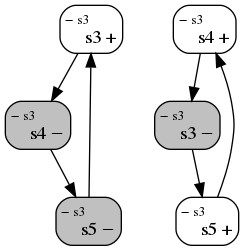
\includegraphics{implication_network.png}
\caption{title}
\end{figure}

\texttt{implication\_network.png}

    Recalling the list of PCUs above, we can see each PCU represented twice
in the implication network above. For example,
\texttt{{[}\textquotesingle{}poss3\_s3\textquotesingle{},\ \textquotesingle{}poss3\_s4\textquotesingle{}{]}}
translates to saying that the following combination of species responses
is impossible in the model: positive s3 and positive s4. Therefore a
positive response in s3 implies a negative response in s4 (seen in
left-hand subnetwork), and a positive response in s4 implies a negative
response in s3 (seen in right-hand subnetwork).

Another function is available, \texttt{draw\_implication\_network2}, to
draw the implication network with only one implication per PCU. One can
specify which species responses they wish to see as the antecedents. The
example below also shows some of its other options.

    \begin{Verbatim}[commandchars=\\\{\}]
{\color{incolor}In [{\color{incolor}37}]:} \PY{k+kn}{from} \PY{n+nn}{findpcu} \PY{k}{import} \PY{n}{draw\PYZus{}implication\PYZus{}network2}
         
         \PY{c+c1}{\PYZsh{} make a positive response of s3 always an antecedent}
         \PY{n}{alwaysAnteList} \PY{o}{=} \PY{p}{[}\PY{l+s+s1}{\PYZsq{}}\PY{l+s+s1}{poss3\PYZus{}s3}\PY{l+s+s1}{\PYZsq{}}\PY{p}{,} \PY{l+s+s1}{\PYZsq{}}\PY{l+s+s1}{negs3\PYZus{}s5}\PY{l+s+s1}{\PYZsq{}}\PY{p}{,} \PY{l+s+s1}{\PYZsq{}}\PY{l+s+s1}{negs3\PYZus{}s4}\PY{l+s+s1}{\PYZsq{}}\PY{p}{]} 
         
         \PY{n}{niceNames} \PY{o}{=} \PY{p}{\PYZob{}} \PY{c+c1}{\PYZsh{} names of each species}
             \PY{l+s+s1}{\PYZsq{}}\PY{l+s+s1}{s3}\PY{l+s+s1}{\PYZsq{}}\PY{p}{:} \PY{l+s+s1}{\PYZsq{}}\PY{l+s+s1}{species 3}\PY{l+s+s1}{\PYZsq{}}\PY{p}{,}
             \PY{l+s+s1}{\PYZsq{}}\PY{l+s+s1}{s4}\PY{l+s+s1}{\PYZsq{}}\PY{p}{:} \PY{l+s+s1}{\PYZsq{}}\PY{l+s+s1}{species 4}\PY{l+s+s1}{\PYZsq{}}\PY{p}{,}
             \PY{l+s+s1}{\PYZsq{}}\PY{l+s+s1}{s5}\PY{l+s+s1}{\PYZsq{}}\PY{p}{:} \PY{l+s+s1}{\PYZsq{}}\PY{l+s+s1}{species 5}\PY{l+s+s1}{\PYZsq{}}\PY{p}{,}
         \PY{p}{\PYZcb{}}
         
         \PY{n}{fName} \PY{o}{=} \PY{l+s+s1}{\PYZsq{}}\PY{l+s+s1}{implication\PYZus{}network\PYZus{}2}\PY{l+s+s1}{\PYZsq{}} \PY{c+c1}{\PYZsh{} name of the .dot file and .pdf file}
         
         \PY{n}{controlSymbol} \PY{o}{=} \PY{l+s+s1}{\PYZsq{}}\PY{l+s+s1}{\PYZam{}\PYZsh{}9785;}\PY{l+s+s1}{\PYZsq{}} \PY{c+c1}{\PYZsh{} html code for a sad face}
         
         \PY{n}{draw\PYZus{}implication\PYZus{}network2}\PY{p}{(}\PY{n}{PCUList}\PY{p}{,} 
                                   \PY{n}{alwaysAnteList}\PY{p}{,} 
                                   \PY{n}{fName}\PY{p}{,} 
                                   \PY{n}{niceNames}\PY{p}{,} 
                                   \PY{n}{controlSymbol}\PY{p}{)}
         
         \PY{n}{os}\PY{o}{.}\PY{n}{system}\PY{p}{(}\PY{l+s+s2}{\PYZdq{}}\PY{l+s+s2}{dot \PYZhy{}Tpng implication\PYZus{}network\PYZus{}2.dot \PYZgt{} implication\PYZus{}network\PYZus{}2.png}\PY{l+s+s2}{\PYZdq{}}\PY{p}{)}
\end{Verbatim}


    \begin{Verbatim}[commandchars=\\\{\}]
implication\_network\_2.pdf has been created

    \end{Verbatim}

\begin{Verbatim}[commandchars=\\\{\}]
{\color{outcolor}Out[{\color{outcolor}37}]:} 0
\end{Verbatim}
            
    \begin{figure}
\centering
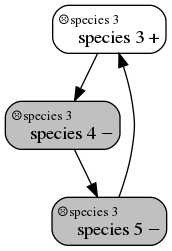
\includegraphics{implication_network_2.png}
\caption{title}
\end{figure}

\texttt{implication\_network\_2.png}


    % Add a bibliography block to the postdoc
    
    
    
    \end{document}
